\documentclass[11pt, ]{article}
\title{An Unusual AKI}
\author{Robert K. Forsythe}
\usepackage{todo}
\usepackage{graphicx}
\usepackage{subcaption}
\graphicspath{ {./images/} }


\usepackage[backend=bibtex,style=numeric,autocite=superscript,natbib=true,sorting=none]{biblatex} 
\addbibresource{Refs.bib}

\begin{document}
\maketitle
\begin{abstract}
	Acetazolamide is a medication prescribed frequently for various indications including idiopathic intracranial hypertension, prophylaxis of mountain sickness and ventilator alkalosis. We here describe an unusual case of drug induced acute kidney injury secondary to acetazolamide. 
\end{abstract}
		
\section*{Case Report}

This 72 year old lady attended the emergency department complaining of right sided loin pain for the past 36 hours. She had a medical history of hyperparathyroidism, hypothyroidism and a rectocele repaired 6 years ago. 48 hours prior to her attendance she had repair of a macular hole and following this had been prescribed acetazolamide 250mg twice daily. She had taken 5 doses of this before discontinuing the medication due to nausea, vomiting and loin pain. She then attended A\&E. Blood tests on attendance demonstrated reduced renal function with a creatinine of 222umol/L from a baseline of around 70umol/L. Initially she was assessed with a non-contrast CTKUB. This did not demonstrate any nephrolithiasis but did suggest some fullness of the collecting system. Given the CT findings she was further assessed with a renal tract ultrasound which excluded any hydronephrosis. 

Unfortunately her renal function continued to decline and a line was placed and 4 days following admission she was dialysed. Her renal function then made a very rapid recovery and she entered a polyuric phase. 

\begin{figure}
\begin{subfigure}{.5\textwidth}
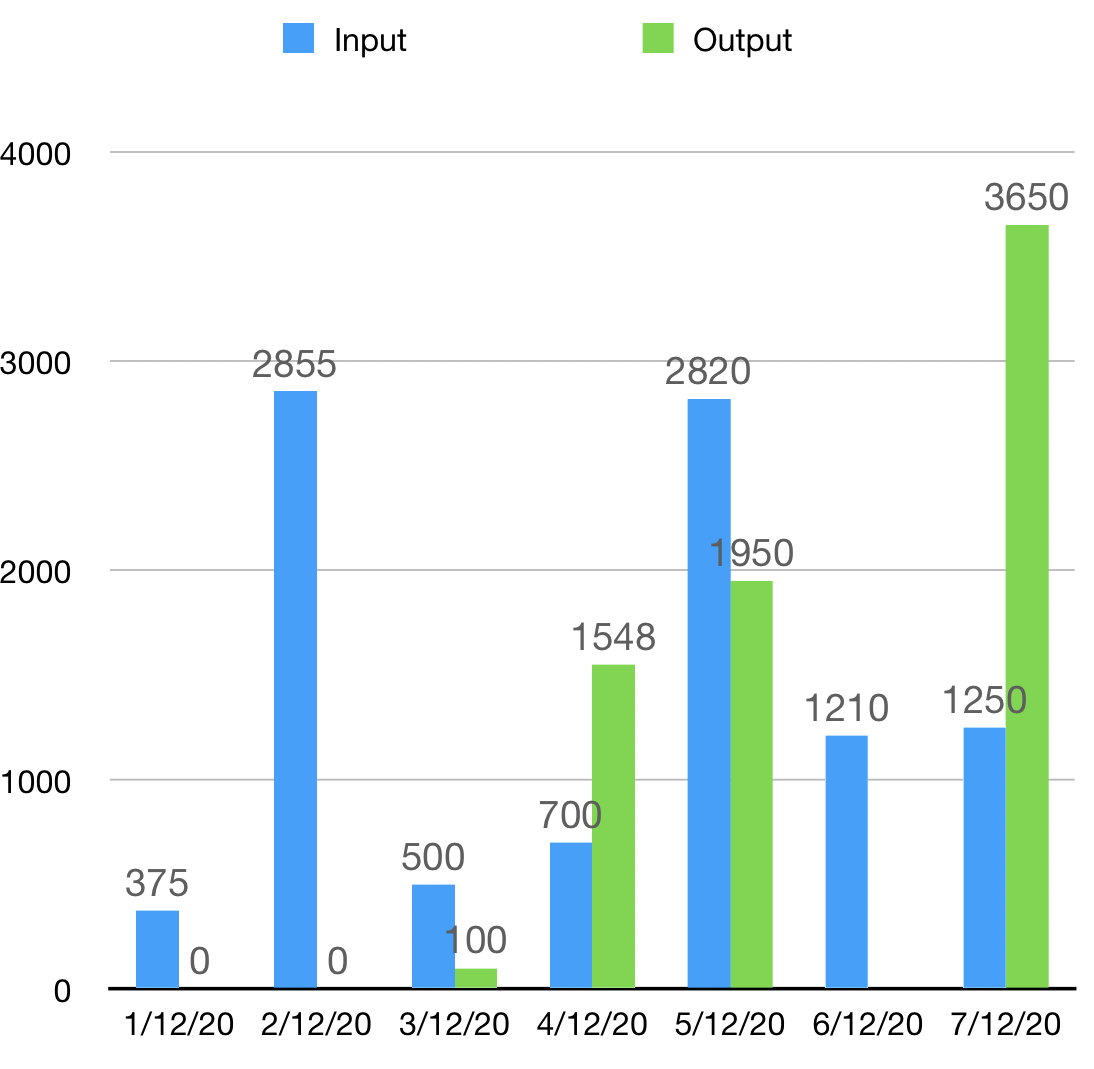
\includegraphics[width=\textwidth]{InputOutput}
\caption{Graph of Daily Fluid Balance}
\end{subfigure}
\begin{subfigure}{.5\textwidth}
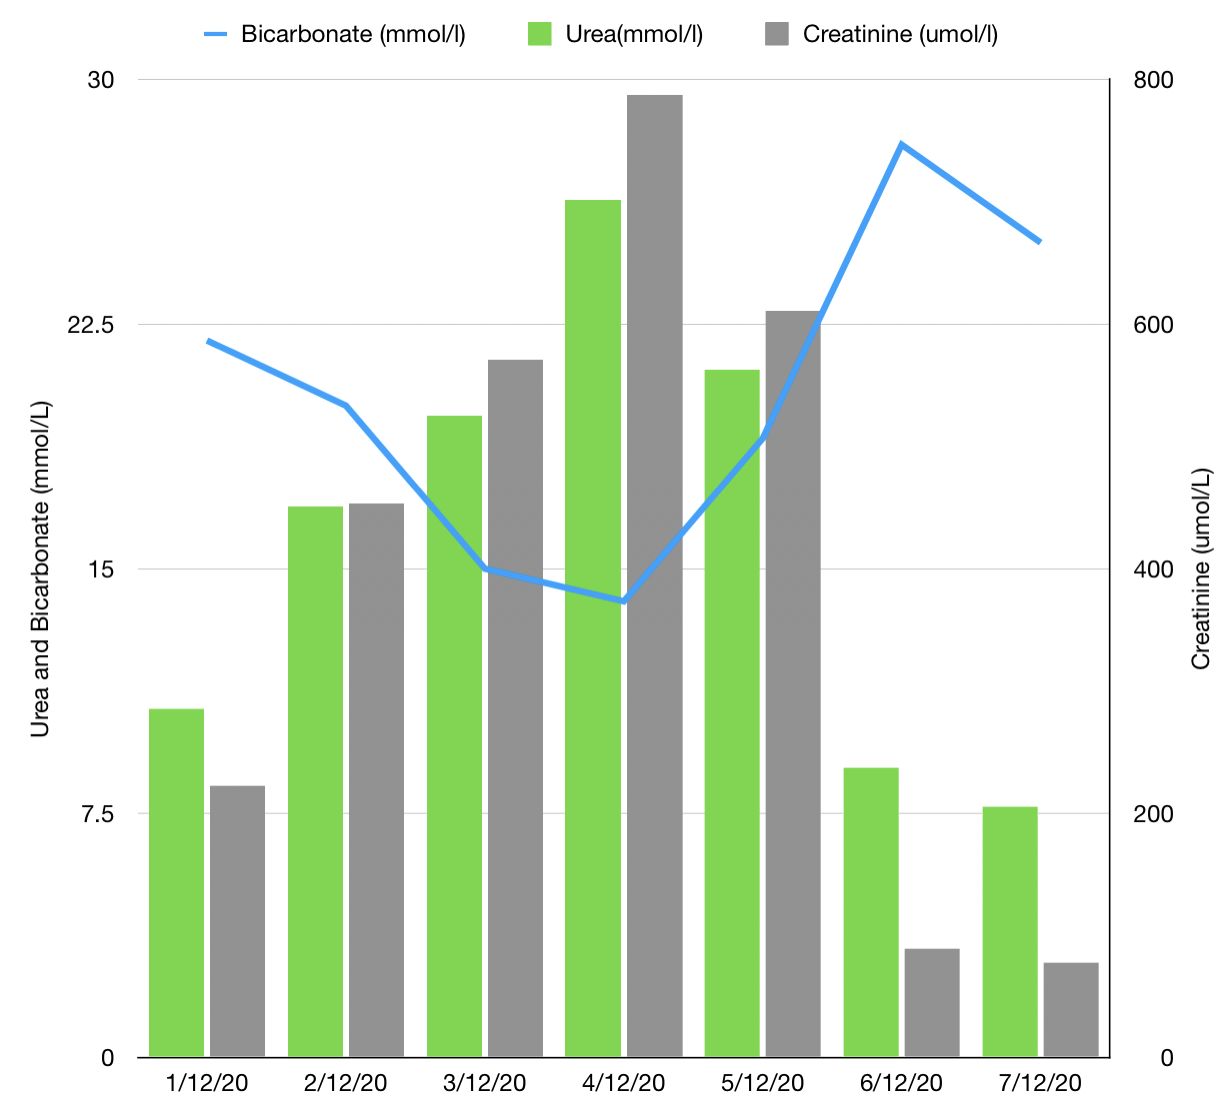
\includegraphics[width=\textwidth]{ubc}
\caption{Graph of Daily Biochemistry}
\end{subfigure}
\end{figure}



\section*{Discussion}
A brief review of the literature demonstrated that similar presentations of acute kidney injury have previously been encountered in assocation with acetazolamide\cite{Neyra2014, Rossert1984, Lawson2020}. In each of these cases acetazolamide has been associated with renal colic and anuria. Lawson found that the AKI demonstrated with aggressive fluid therapy and Neyra's patient required 2 sessions of haemodialysis. Acetazolamide is recognised to be associated with metabolic drug-induced calcium phophate or oxalate calculi, however in this case these were excluded by CT imaging. An older case published by Rossert in 1989 describes a similar case in which a biopsy was performed and demonstrated Tamm-Horsfall protein within the glomeruli and tubular lesions associated with intratubular crystal formation.This suggests intratubular obstruction and retrograde flow of tubular urine\cite{Rossert1984}.  




\printbibliography
\end{document}
